\documentclass[12pt,a4paper]{report}
\usepackage[utf8]{inputenc}
\usepackage{amsmath}
\usepackage{amsfonts}
\usepackage{amssymb}
\usepackage{amsthm}
\usepackage{hyperref}

\usepackage{multicol}
\usepackage{fancyhdr}
\usepackage[inline]{enumitem}
\usepackage{tikz}
\usepackage{tikz-cd}
\usetikzlibrary{calc}
\usetikzlibrary{shapes.geometric}
\usetikzlibrary{positioning}
\usepackage[margin=0.5in]{geometry}
\usepackage{xcolor}

\hypersetup{
    colorlinks=true,
    linkcolor=blue,
    filecolor=magenta,      
    urlcolor=cyan,
    pdftitle={Tensors},
    pdfpagemode=FullScreen,
    }

%\urlstyle{same}

\newcommand{\CLASSNAME}{Math 5050 -- Special Topics: Tensor Analysis}
\newcommand{\STUDENTNAME}{Paul Carmody}
\newcommand{\ASSIGNMENT}{Chapter 3: Coordinate Systems and the Role of Tensor Calculus }
\newcommand{\DUEDATE}{January 2026}
\newcommand{\PROFESSOR}{Professor Berchenko-Kogan}
\newcommand{\SEMESTER}{Spring 2026}
\newcommand{\SCHEDULE}{TBD}
\newcommand{\ROOM}{Remote}

\newcommand{\MMN}{M_{m\times n}}
\newcommand{\FF}{\mathcal{F}}

\pagestyle{fancy}
\fancyhf{}
\chead{ \fancyplain{}{\CLASSNAME} }
%\chead{ \fancyplain{}{\STUDENTNAME} }
\rhead{\thepage}

\fancyfoot{} % clear all footer fields
\fancyfoot[LE,RO]{\thepage}
\fancyfoot[LO,CE]{-------\\\ASSIGNMENT}
%\fancyfoot[CO,RE]{To: Dean A. Smith}
\input{../MyMacros}

\newcommand{\RED}[1]{\textcolor{red}{#1}}
\newcommand{\BLUE}[1]{\textcolor{blue}{#1}}

\newcommand{\SUPP}{\operatorname{supp}}
\newcommand{\CLOSURE}{\operatorname{closure of}}
\newcommand{\BD}{\operatorname{bd}}
\newcommand{\HHN}{\mathcal{H}^n}
\newcommand{\COFF}[3]{\Gamma^{#1}_{{#2}{#3}}}
\newcommand{\VK}[1]{\textbf{#1}}
\newcommand{\VKR}{\VK{R}}
\newcommand{\VKZ}{\VK{Z}}

\begin{document}

\begin{center}
	\Large{\CLASSNAME -- \SEMESTER} \\
	\large{ w/\PROFESSOR}
\end{center}
\begin{center}
	\STUDENTNAME \\
	\ASSIGNMENT -- \DUEDATE\\
\end{center} 

\textbf{Exercises}
\begin{enumerate}[label=\textbf{\arabic*.}]
\setcounter{enumi}{18}
%Section 3.6
\item Generalize the content of the section to three dimension.

\item Describe a set of six degrees of freedom in choosing Cartesian coordinates in the three-dimensional space.

\item Given a polar coordinate system, introduce Cartesian coordinates that originate at the same pole and for which the $x$-axis coincides withthe polar axis.  Show that the Cartesian coordinates $(x,y)$ are related to the polar coordinates $(r,\theta)$ by the following identities:
\begin{align*}
	x(r,\theta) = r\cos \theta \\
	y(r,\theta) = r\sin \theta
\end{align*} 
\begin{center}

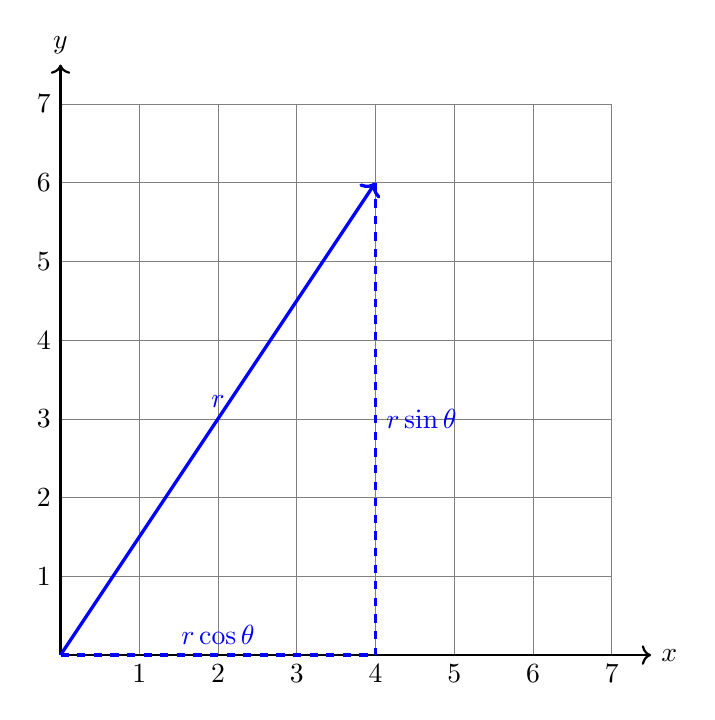
\begin{tikzpicture}
    % 1. Draw the grid with light gray, thin lines and 1cm step size
    \draw[step=1cm, gray, very thin] (0,0) grid (7,7);

    % 2. Draw the axes (optional, but helpful for context)
    \draw[->, thick] (0,0) -- (7.5,0) node[right] {$x$};
    \draw[->, thick] (0,0) -- (0,7.5) node[above] {$y$};

    % 3. Add coordinates for context (optional)
    \foreach \x in {1, 2, 3, 4, 5, 6, 7} {
        \node[below] at (\x, 0) {$\x$};
    }
    \foreach \y in {1, 2, 3, 4, 5, 6, 7} {
        \node[left] at (0, \y) {$\y$};
    }

    % 4. Draw a vector from the origin (0,0) to the point (3, 2)
    % The "->" option creates an arrow head
    \draw[->, very thick, blue] (0,0) -- (4,6) node[midway, above ] {$r$};

    % 4. Draw a vector from the origin (0,0) to the point (3, 2)
    % The "->" option creates an arrow head
    \draw[dashed, very thick, blue] (4,6) -- (4,0) node[midway, right ] {$r\sin \theta$};    

    % 4. Draw a vector from the origin (0,0) to the point (3, 2)
    % The "->" option creates an arrow head
    \draw[dashed, very thick, blue] (0,0) -- (4,0) node[midway, above ] {$r\cos \theta$};    
\end{tikzpicture}
\end{center}


\item Show that the inverse relationship is
\begin{align*}
	r(x,y) &= \sqrt{x^2+y^2} \\
	\theta(x,y) &= \arctan \frac{y}{x}
\end{align*}

\BLUE{\begin{align*}
	x(r,\theta)^2 + y(r, \theta)^2 &= r^2\cos^2\theta+r^2\sin^\theta = r^2 \implies r(x,y) = \sqrt{x^2+y^2}  \\
	\tan \theta &= \frac{\sin\theta}{\cos\theta} = \frac{r\sin\theta}{r\cos\theta} \frac{y}{x} \implies \theta = \arctan\frac{y}{x}
\end{align*}
}

\item Align a Cartesian coordinate system $x,y,z$ with a given cylindrical coordinate system in a natural way.  Show that $x,y,z$ and $r, \theta, z$ (we hop it is OK to reuse the letter $z$) are related as follows
\begin{align*}
	x(r,\theta,z) &= r\cos \theta\\
	y(r,\theta,z) &- \arctan\frac{y}{x} \\
	z(x,y,z) &= z
\end{align*}

\BLUE{Given cylindrical coordinates $(r, \theta, z)$, we can make Cartesian coordinates $(x,y,z)$ where the $x$-axis cooresponds to $\theta = 0$ and the $z$-axis is the same in both.  Consequently, as in 21 above, any point $p=(r, \theta)$  will have projections onto the $x$ and $y$ axes as 
\begin{align*}
	x(r, \theta, z) &= r\cos \theta \\
	y(r, \theta, z) &= r\sin \theta \\
	z(r, \theta, z) &= z.
\end{align*}Alternatively, we can envision a vector $\VK{P} = (r, \theta)$ projected onto the $x$-axis with the unit vector $\hat{i}$.  $\VK{P} \cdot \hat{i} = |\VK{P}|\,|\hat{i}|\cos\theta = r\cos\theta$. And similarly for the unit vector of the $y$-axis, $\hat{j}$.
}

\item Align a Cartesian coordinate system with a spherical coordinate system in a natural way.  Show that $x,y, z$ and $r,\theta,\phi$ are related by
\begin{align*}
	x(r,\theta, \phi) &= r\sin\theta\cos \phi\\
	y(r, \theta, \phi) &= r\sin\theta\sin\phi \\
	z(r, \theta, \phi) &= r\cos \phi
\end{align*}

\BLUE{``Align in a natural way", let the two coordinate systems have the same origin and let the polar axis be $z$, $\theta$ be the angle made between the line connecting the point to the origin and $z$.  Then $z=r\cos\theta$.  Project this line into the $x-y$ plane producing the angle $\phi$ from the $x$ axis.  The length of this projection is $r\sin\theta$ and giving us $x=r\sin\theta\cos\phi$ and $y=r\sin\theta\sin\phi$
}

\item show that the inverse relationship is 
\begin{align*}
	r(x,y,z) &= \sqrt{x^2+y^2+z^2}\\
	\theta(x,y,z) &= \arcsin\frac{z}{\sqrt{s^2+y^2+z^2}} \\
	\phi(x,y,z) &= \arctan\frac{y}{x}
\end{align*}
\end{enumerate}
\end{document}